\subsection{Test Case Instance - instance01Part02}


%%%%%%%%%%%%%%%%%%%%%%%%%%%%%%%%%%%%%%%%%%%%%%%%%%
%Test Step Instances
%%%%%%%%%%%%%%%%%%%%%%%%%%%%%%%%%%%%%%%%%%%%%%%%%%


Figure \ref{fig:lu.uni.lassy.excalibur.examples.icrash-TM-instanceview-tci-testcase01-instance01-Part02}
Sequence diagram representing the second part of a simple and complete testcase instance for \msricrash.

\begin{figure}[htbp]
\begin{center}

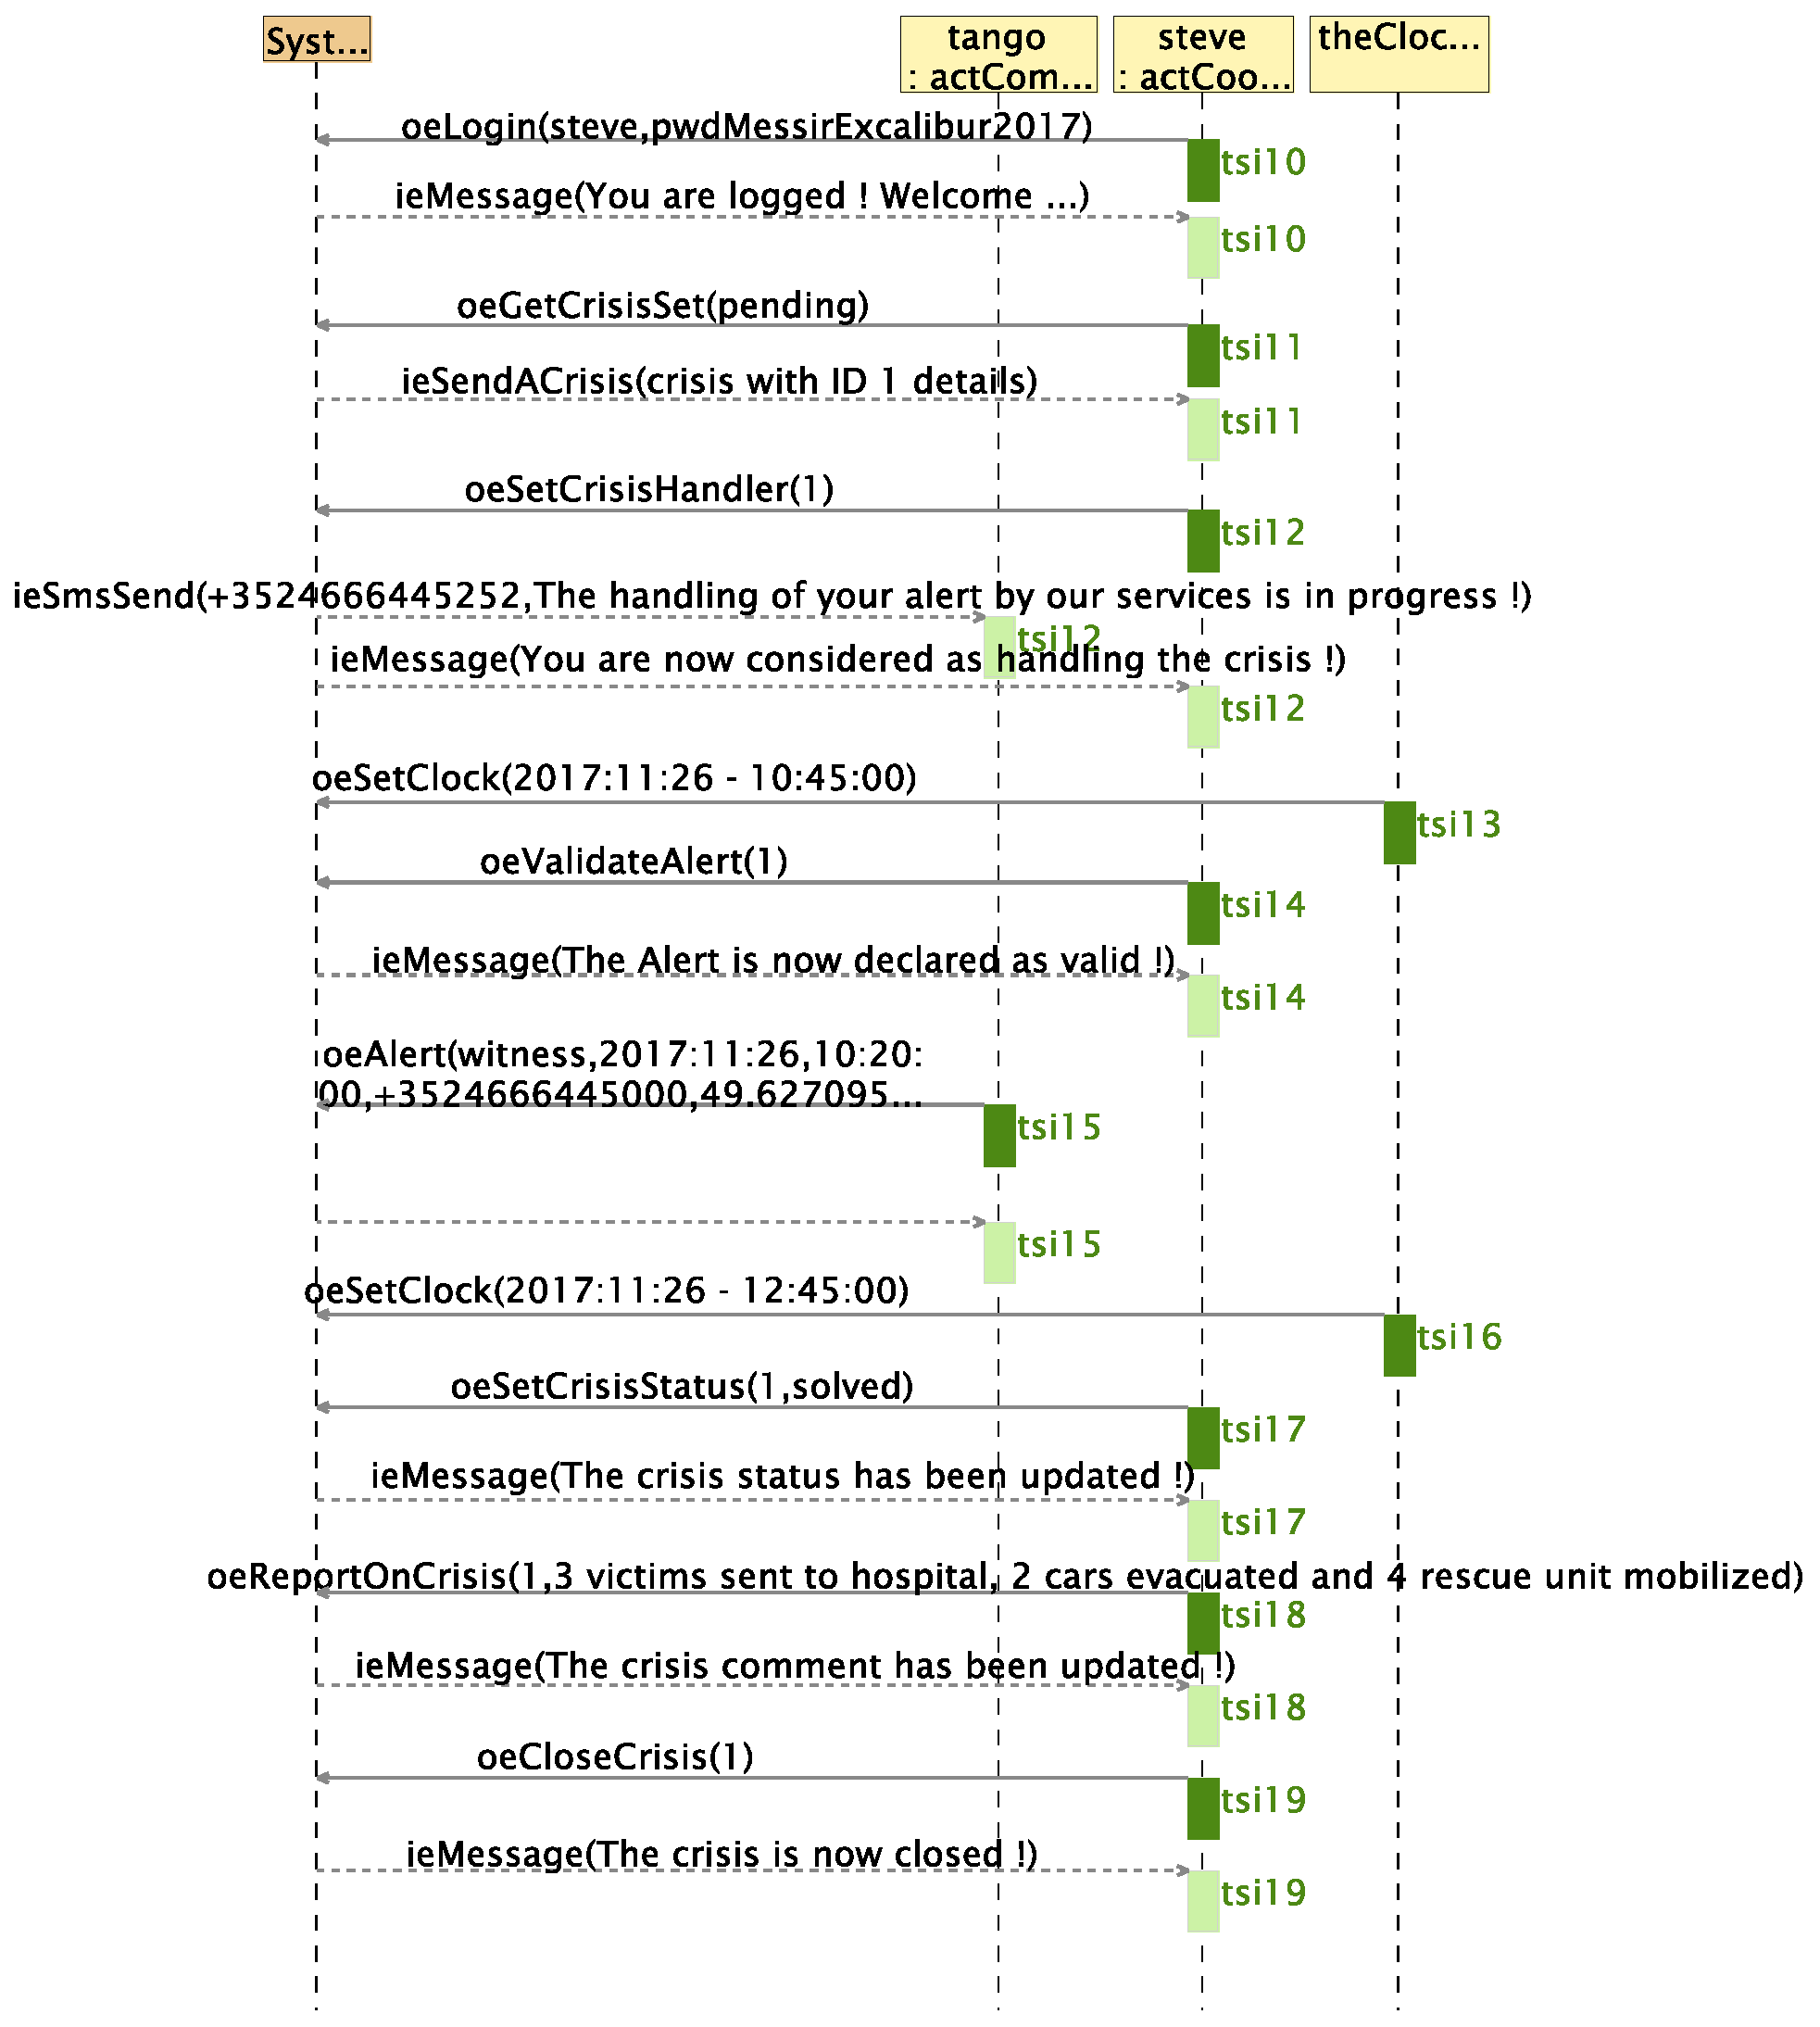
\includegraphics[angle=0
,height=1.0\textheight
]{./images-report-gen/testcase-model/tci-testcase01-instance01-Part02.eps}
\end{center}
\caption[lu.uni.lassy.excalibur.examples.icrash Sequence Diagram: tci-testcase01-instance01-Part02]{tci-testcase01-instance01-Part02 testcase instance sequence diagram
}
\label{fig:lu.uni.lassy.excalibur.examples.icrash-TM-instanceview-tci-testcase01-instance01-Part02}
\end{figure}
\vspace{0.5cm}
